%UNDERSTANDING AREA \& UNIT SQUARES - WORKSHEET 0 (IN-CLASS INSTRUCTION)
\documentclass[12pt, letterpaper, fleqn]{article}

% ----------------------------------------------------------
% PACKAGES
% ----------------------------------------------------------
\usepackage{graphicx}
\usepackage{xcolor}
\usepackage[most]{tcolorbox}
\usepackage{amsmath, amssymb}
\usepackage{fancyhdr}
\usepackage[utf8]{inputenc}
\usepackage[T1]{fontenc}
\usepackage{enumitem}
\usepackage{geometry}
\usepackage{tikz}
\usepackage{needspace}
\usepackage{multicol}

\usetikzlibrary{arrows.meta, calc, shapes.geometric}

% ----------------------------------------------------------
% PAGE SETUP
% ----------------------------------------------------------
\usepackage{times}
\geometry{letterpaper, top=1.25in, bottom=1.25in, marginpar=0.5in}

% ----------------------------------------------------------
% HEADER / FOOTER
% ----------------------------------------------------------
\newcommand{\logowidth}{3cm}
\setlength{\headheight}{20pt}
\setlength{\footskip}{40pt}

\pagestyle{fancy}
\fancyhf{}
\fancyhead[C]{\small\bfseries Understanding Area \& Unit Squares}
\fancyfoot[L]{\raisebox{2pt}{
\includegraphics[width=\logowidth]{../kss.png}}}
\fancyfoot[C]{\thepage}
\fancyfoot[R]{3.22.0}

\renewcommand{\footrulewidth}{0.2pt}

% ----------------------------------------------------------
% THEME COLOR
% ----------------------------------------------------------
\definecolor{customteal}{HTML}{2fbdb9}

% ----------------------------------------------------------
% HELPER MACROS
% ----------------------------------------------------------
\newcommand{\blank}{\underline{\hspace{2.2cm}}}
\newcommand{\blanklong}{\underline{\hspace{6.5cm}}}
\newcommand{\blankshorter}{\underline{\hspace{1.5cm}}}

% ----------------------------------------------------------
% DOCUMENT
% ----------------------------------------------------------
\begin{document}

\textbf{Name:} \underline{\hspace{5cm}}
\hfill
\textbf{Date:} \underline{\hspace{3cm}}\\

\begin{tcolorbox}[colback=customteal!20]
    \large\textcolor{black}{\textbf{Understanding Area & Unit Squares}}
\end{tcolorbox}

\vspace{3mm}
\noindent
**Area** is the amount of flat space inside a shape. 
We measure area in **square units** by counting how many **unit squares** fit inside without gaps.

\begin{tcolorbox}[colback=white, colframe=black!25, boxrule=0.6pt, arc=4mm]
\textbf{Grid Model}
\begin{center}
\begin{tikzpicture}[scale=0.8]
\draw[step=1cm,gray,very thin] (0,0) grid (4,3);
\draw[thick] (0,0) rectangle (4,3);
\fill[customteal!30] (1,1) rectangle (3,3);
\draw[step=1cm,gray,very thin] (0,0) grid (4,3); % Redraw grid lines
\draw[thick] (0,0) rectangle (4,3); % Redraw outline
\end{tikzpicture}
\end{center}
The shaded region has 4 squares inside. Its area is **4 square units**.
\end{tcolorbox}

\newpage
\begin{tcolorbox}[colback=customteal!20]
    \large\textcolor{black}{\textbf{Guided Practice}}
\end{tcolorbox}

\vspace{5mm}
\noindent
Count the unit squares to find the area of the shapes.

\vspace{8mm}
\begin{enumerate}[itemsep=3.5cm, leftmargin=0.6cm]
\item 
\begin{tikzpicture}[scale=0.8]
\draw[step=1cm,gray,very thin] (0,0) grid (3,3);
\fill[customteal!30] (0,0) rectangle (3,2);
\draw[step=1cm,gray,very thin] (0,0) grid (3,3);
\draw[thick] (0,0) rectangle (3,3);
\end{tikzpicture}
\\
Area: \blank square units

\item 
\begin{tikzpicture}[scale=0.8]
\draw[step=1cm,gray,very thin] (0,0) grid (4,2);
\fill[customteal!30] (0,0) rectangle (4,2);
\draw[step=1cm,gray,very thin] (0,0) grid (4,2);
\draw[thick] (0,0) rectangle (4,2);
\end{tikzpicture}
\\
Area: \blank square units
\end{enumerate}

\end{document}
